% !TeX TS-program = xelatex

\documentclass{beamer}
%Set the slide theme
%Change to meet your taste
% Madrid, Copenhagen, Berlin, ... works
%\usetheme{Copenhagen} 
\usetheme{CambridgeUS}
\usepackage{graphicx}
\usepackage{xecolor}
\usepackage{amsmath}
%\usefonttheme[onlymath]{serif} %Change the math font

\usepackage{xepersian}
\settextfont{XB Niloofar}




%---------------------------------------------------------------------------------
% Seetings to force Beamer works with Xepersian and RTL typesetting
%-------------------------------------------------------------------------------
%\raggedleft

% For right to left lists (itemize and enumerate)
\makeatletter
\newcommand{ \RTList}{\raggedleft\rightskip\@totalleftmargin} 
\makeatother
% Correct the bullet for RTL texts
\setbeamertemplate{itemize item}{\scriptsize\raise1.25pt%
 \hbox{\donotcoloroutermaths$\blacktriangleleft$}} 

% To force beamer use numbering in captions
\setbeamertemplate{caption}[numbered]{}% Number float-like environments

%---------------------------------------------------------------------------------
\title{
جداسازی کور ترکیب‌های غیرخطی فرآیند‌های تصادفی
}

\author[بهراد منیری]{
	بهراد منیری\\
\footnotesize\url{bemoniri@ee.sharif.edu} \\\vspace{0.5cm}
استاد راهنما:\\
دکتر مسعود بابائی‌زاده}


\institute[دانشگاه‌ صنعتی شریف]{
دانشکده‌ی مهندسی برق\\
دانشگاه صنعتی شریف
}


\date{\today}
\newtheorem{den}{{\large\bf تعریف}}[section]
\newtheorem{lem}{{\large\bf لم}}[section]
\newtheorem{pro}{{\large\bf گزاره}}[section]
\newtheorem{cor}{{\large\bf نتیجه}}[section]
\newtheorem{thm}{{\large\bf قضیه}}[section]
\newtheorem{rem}{{\large\bf تذکر}}[section]
\newtheorem{nnt}{{\large\bf توجه}}[section]
\newtheorem{aaa}{{\large\bf}}[section]

\begin{document}
\begin{persian}
%------------------------------------------
% Title page
%------------------------------------------
\begin{frame}
\maketitle
\end{frame}

% To adjust the paragraphs in RTL
\everypar{\rightskip\rightmargin}
%-------------------------------------------------------------------------------
\begin{frame}{جداسازی کور منابع}
\frametitle{جداسازی کور منابع: معرفی مسئله}

\begin{figure}
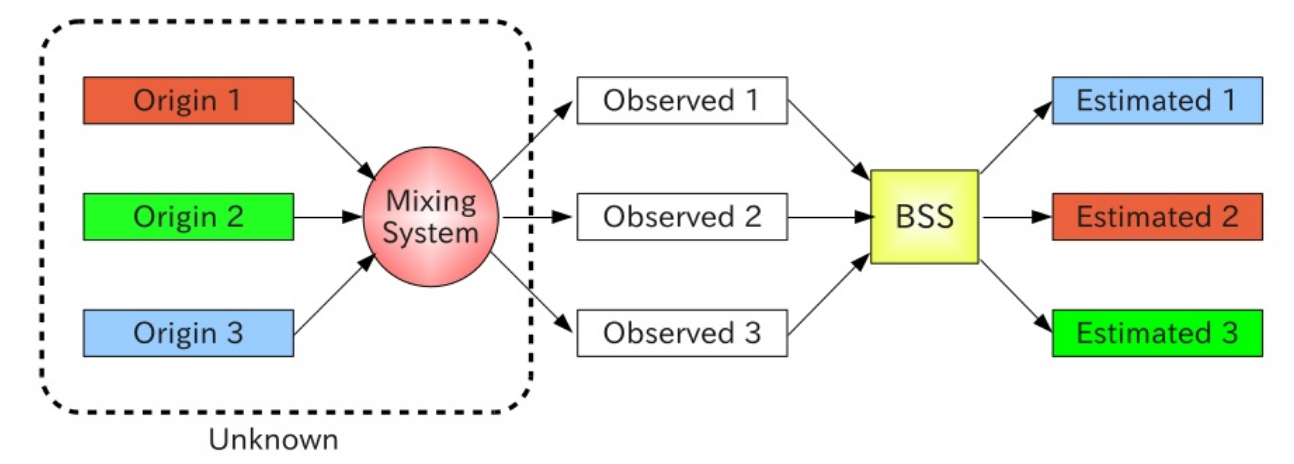
\includegraphics[scale=0.25]{slide1.png}
\end{figure}

\end{frame}

%-------------------------------------------------------------------------------

%-------------------------------------------------------------------------------
\section{معرفی مسئله}
\begin{frame}
\frametitle{نتایج پیشین: ترکیب‌های خطی}

\begin{itemize}\RTList
\item
\textbf{	تحلیل مولفه‌های مستقل (ICA) خطی برای متغیر‌های تصادفی غیرگوسی}
$$
\textbf{x} = A\textbf{s} \implies
\begin{bmatrix}
x_1\\x_2\\\vdots\\x_n
\end{bmatrix}
= 
\begin{bmatrix}
a_{11}&a_{12}&\dots&a_{1n}\\
a_{21}&a_{21}&\dots&a_{2n}\\
\vdots&\vdots&\ddots&\vdots\\
a_{n1}&a_{n1}&\dots&a_{nn}\\
\end{bmatrix}
\begin{bmatrix}
s_1\\s_2\\\vdots\\s_n
\end{bmatrix}
\implies
\textbf{s} = A^{-1} \textbf{x}
 $$
\begin{center}
	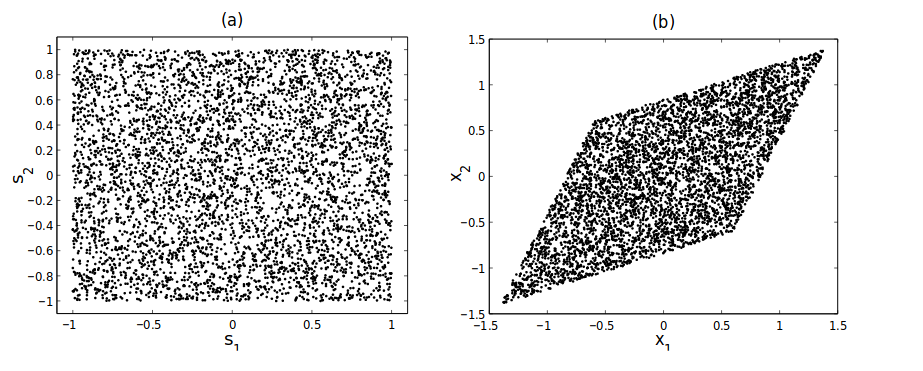
\includegraphics[scale=0.25]{linica.png}
\end{center}


\item
الگوریتم‌های 
\lr{Fast-ICA}
و
\lr{EASI}.

\end{itemize}
\end{frame}

\begin{frame}
\frametitle{نتایج پیشین: ترکیب‌های غیرخطی}
\begin{itemize}\RTList
	\item
در ترکیب‌های غیرخطی متغیر‌های تصادفی، جداسازی غیرممکن است:
\begin{equation}
\begin{cases}
S_1 = \mathrm{Uniform} [0, 2\pi]\\
S_2 = \mathrm{Rayleigh}(\sigma)
\end{cases}
\implies
S_2 \cos (S_1) \perp \!\!\! \perp  S_2 \sin (S_1)
\end{equation}

\end{itemize}
\end{frame}


\begin{frame}
\frametitle{نتایج پیشین: فرآیند‌های تصادفی}
\begin{itemize}\RTList
	\item
		\lr{[Harmeling et al., 2003]}:
پیشنهاد استفاده از ارتباط‌های زمانی برای جداسازی (استفاده از استقلال فرآیند‌های تصادفی به جای استقلال متغیر‌های تصادفی)
	
	\item
	\lr{[Hyvarinen et al, 2017]}:
ترکیب‌های غیرخطی فرآیند‌های تصادفی قابل جداسازی هستند.
\begin{thm}
	 فرض کنید 
	 $\textbf{x}(t) = \textbf{f}\big(\textbf{s}(t)\big)$
	 باشد. این ترکیب قابل جداسازی است، اگر:
	 \begin{itemize}
	 	\item
	 	تابع 
	 	$\textbf{f}$
	 	وارون‌پذیر، و هموار باشد.
	 	\item
	 	فرآیند‌های تصادفی 
	 	$s_i(t)$
	 	مستقل، ایستان و ارگودیک باشد.
	 	\item
	 	شرایطی «مشابه» گوسی نبودن بر روی فرآیند‌های تصادفی برقرار باشد
	 	\item
           وجود رابطه‌های زمانی «قوی» در فرآیند‌های تصادفی برقرار باشد.
           
	 \end{itemize}

      \end{thm}
\end{itemize}
\end{frame}

%-------------------------------------------------------------------------------
\begin{frame}{اهداف پروژه}
\begin{itemize}\RTList
\item
من بعد از بررسی اثبات 
	\lr{Hyvarinen et al.}
	در مقاله‌ی سال ۲۰۱۷ متوجه ایرادی در اثبات شدم. بررسی آثار آن و همچنین اصلاح آن بخشی از پروژه‌ی من است.
\item
آیا شرایط وضع شده بر روی فرآیند‌های تصادفی ورودی محدود کننده‌اند؟  یافتن دسته‌ای از فرآیند‌ها با شرط فوق.
\item
الگوریتمی برای جداسازی ترکیب‌ها بر مبنای کمینه‌ کردن اطلاعات متقابل فرآیند‌های تصادفی خروجی.
\item
 استفاده از این تئوری جدید برای حل مسائل کاربردی

\end{itemize}
\end{frame}


%-------------------------------------------------------------------------------
\begin{frame}{کاربرد‌های احتمالی}
\frametitle{حذف رد پشت برگه در تصاویر اسکن شده}
\begin{figure}
	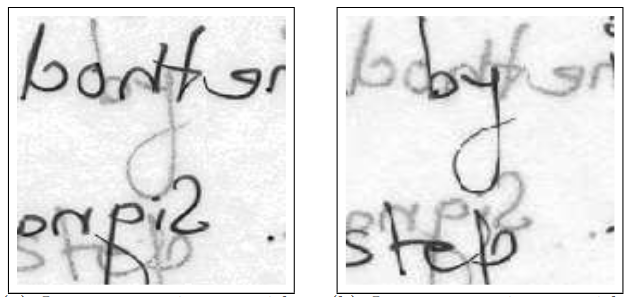
\includegraphics[scale=0.5]{application1.png}

\end{figure}
\end{frame}

\begin{frame}
\frametitle{پیش پردازش سیگنال الکتروانسفالوگرام}
\begin{figure}
	\includegraphics[scale=0.3]{brain.png}
\end{figure}
\end{frame}
\begin{frame}
\frametitle{مراجع}
\nocite{harmeling2003kernel,hyvarinen2017nonlinear,babaie2005general,comon2010handbook}
\begin{latin}
\begin{footnotesize}
\bibliographystyle{chicagoa}
\bibliography{bib}
\end{footnotesize}
\end{latin}
\end{frame}
%-------------
\end{persian}

\end{document}